
\chapter{Podaci i metode} % Main chapter title

\label{Podaci i metode} % For referencing 

Cilj rada je ispitivanje veze između molekulske funkcije proteina i njegove\\ 
(ne)uređenosti tj. da li molekulska funkcija zavisi više od uređenosti ili
neuređenosti. Istraživanje je motivisano radom\parencite{Xie2007}. Navedeni rad
je prvi u seriji od tri rada i bavi se prvenstveno biološkim procesima i
molekulskim funkcijama.  U nastavku teksta pod terminima \keyword{referentni}
rad, autori, podaci, metode i slično podrazumevaćemo navedeni rad, njegove
autore, metode, podatke itd.

Najveća razlika u pristupu između referentnog i ovog istraživanja je što su
referentni rezultati izraženi u terminima \keyword{ključnih
Svis-Prot-reči} (nadalje samo \keyword{ključnih reči}) dok su u ovom
istraživanju rezultati izraženi u \keyword{GO-terminima}. Oba pristupa
proizvode listu funkcija koreliranih sa uređenim, odnosno neuređenim
proteinima, ali GO-termini se zbog granularnosti prirodnije predstavljaju
grafovski jer sadrže za red veličine više funkcija. Jedan od rezultata ovog
istraživanja predstavlja poređenje ova dva pristupa.


\section {Podaci}

Za metode koje prezentujemo potrebne su tri vrste informacija:
\begin{enumerate}
  \item Što više različitih proteina
  \item Pouzdana anotacija funkcija
  \item Informacije o funkcijama, prvenstveno međurelacije (međurelacije između\\ funkcija su bitne  ako ih je potrebno grupisati)
\end{enumerate}


\subsection{Podaci iz referentnog rada}

U referentnom radu \parencite{Xie2007} korišćena je  baza podataka 
\keyword{\swissprot} (Poglavlje \ref{svis-prot}), verzija 48 iz 2005.
Verzija 48 ima 201 560 proteina od kojih 196 326 imaju dužinu preko 40
aminokiselina (što je potrebno zbog Definicije \ref{pdis_def} u nastavku). Funkcije
pridružene proteinima izražene su \keyword{kontrolisanim vokabularom}
\en{controlled vocabulary} koji čine takozvane \textit{UniProtKB} \keyword{ključne reči}
\en{keywords}. U verziji 48, UniProtKB sadrži 874 ključnih reči.  Zbog
statističke značajnosti posmatrane su one ključne reči kojima je bilo anotirano
barem 20 proteina, tj. 710 ključnih reči.

Kao što je pomenuto u Poglavlju \ref{svis-prot}, kanonske sekvence (proteini) iz baze \swissprot
nisu redundantne u smislu da jedan unos u bazi podataka predstavlja produkt
jednog gena iz jedne vrste organizma. Međutim, za analizu funkcija baza
\swissprot \keyword{je statistički redundantna} \parencite{Xie2007} jer
sadrže veliku količinu \keyword{homologih} proteina (prvenstveno ortologa).
Zbog statističke redundantnosti referentni autori su izvršili klasterovanje \swissprot
proteina u \keyword{proteinske familije} dobivši 27 217 familija. Posledica
klasterovanja je da svaki protein dobija težinu kojom doprinosi daljoj analizi.
Težina svakog proteina u preseku klastera sa datom funkcijom je obrnuto
proporcionalna veličini preseka tako da je zbir težina svih proteina jednaka
veličini preseka.

% \textbf{komentar:} \\
% Ono što autori nisu elaborirali jeste da početni uslov od minimum 20 proteina
% po ključnoj reči možda nije dovoljan. Ako pretpostavimo zarad ilustracije
% normalnu raspodelu veličina klastera proteina, očekivali bi da klaster najčešće
% sadrži 7 proteina. Dakle iako je 50 proteina pridruženo nekoj funkciji ona
% verovatno ima pridruženih svega 7 familija proteina. Kako familija sadrži
% proteine pod pretpostavkom istog evolutivnog porekla njihova funkcija bi
% trebalo da je slična pa se onda postavlja pitanje da li je 7 familija dovoljno
% da bi se razmatrala data ključna reč. Ovo je primarno kritika za ključne reči
% jer one obično predstavljaju opšte pojmove.
%
% Sa druge strane za usko specijalizovane pojmove bila bi dovoljna jedna familija
% proteina jer bi ona predstavljala sve razne homologe (TODO Burkhard Rost,
% Termofili)

\subsection{Podaci korišćeni u ovom istraživanju}

Ugledom na \ikeyword{CASP} takmičenja, \ikeyword{CAFA} \en{Critical Assessment of
Functional Annotation} takmičenje pokrenuto je zarad objektivnog ocenjivanja
prediktora funkcije proteina i usmeravanja budućeg razvoja ove oblasti
\parencite{CAFA}.  U ovom radu je korišćen trening skup proteina preuzet sa
\ikeyword{CAFA3} takmičenja, održanog 2017. Trening skupovi su podaci na osnovu
kojih prediktor uči, pa shodno tome ovaj skup treba da predstavlja dobar uzorak
proteina odnosno njihovih funkcija.


Trening skup sa CAFA3 takmičenja (u nastavku samo CAFA3-skup ili CAFA3-podaci) je podskup baze \swissprot (iz 2016.) koji
uključuje proteine iz model organizama: \textit{Human, Mouse, Rat, S.
cerevisiae, S. pombe, E. coli, A. thaliana, Dictyostelium discoideum,
Zebrafish, Bacillus cereus} sa izuzetokm sekvenci \textit{Drosophila} i \textit{Candida}
koje su preuzete iz svojih genomskih baza podataka, respektivno.
Slika \ref{fig:sp_vs_cafa3} pruža detaljan taksonomski uvid o poreklu proteina iz CAFA3-skupa.
Na primer, baza \swissprot sadrži oko 20 000 ljudskih (\textit{Homo})
proteinskih sekvenci dok njen CAFA3-podskup sadrži malo manje od 15 000.  Vrste
koje doprinose sa manje od 100 proteina nisu prikazane radi kompaktnosti.

\begin{figure}[th]
\centering
\hspace*{-3.0cm} 
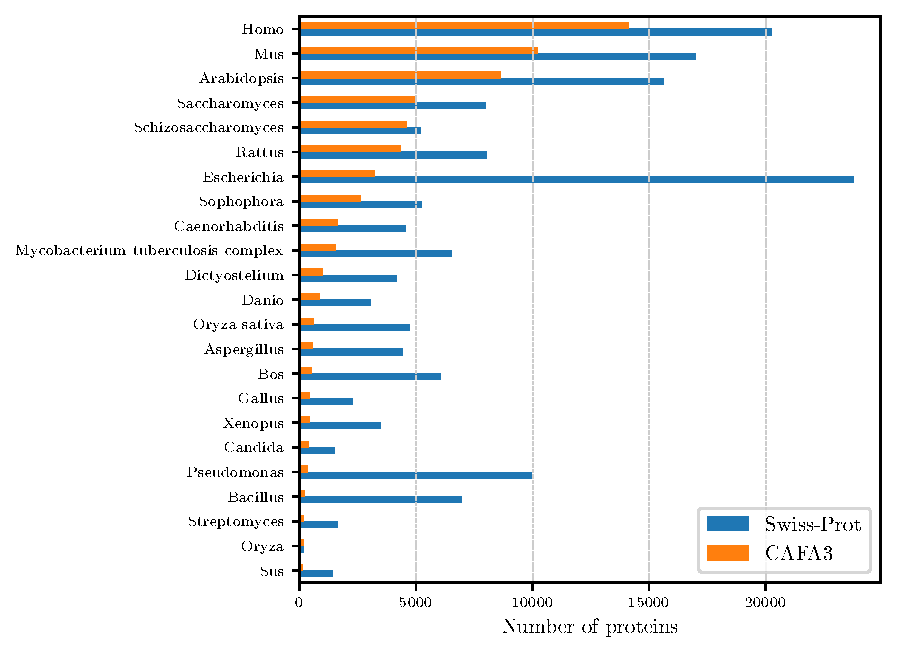
\includegraphics[]{plots/sp_vs_cafa3}
% \decoRule
\caption{Taksonomsko poreklo CAFA3 proteina. \\ \footnotesize 
}
\label{fig:sp_vs_cafa3}
\end{figure}

Za razliku od proteina iz baze \swissprot čije je postojanje pretežno utvrđeno
iz homologije, $74\%$ proteina iz CAFA3-podskupa identifikovani su na 
nivou proteina što je najveći stupanj sigurnosti da proteini zaista postoji. Na
Slici \ref{fig:cafa3_pe} ilustrovana je razlika u odnosu na pouzdanost
postojanja proteina. 



\begin{figure}[th]
\centering
\hspace*{-.1cm} 
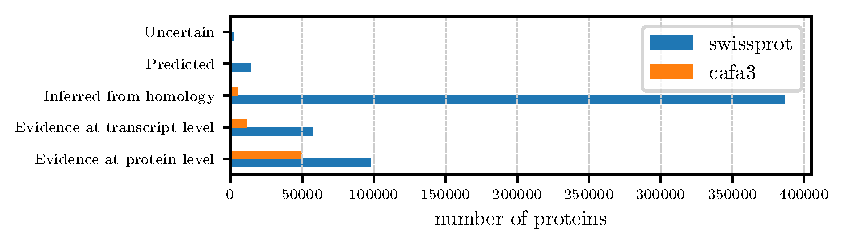
\includegraphics[]{plots/cafa3_pe}
% \decoRule
\caption{Razlika izmedju pouzdanosti postojanja proteina iz \\ baze \swissprot i njenog CAFA3-podskupa. }
\label{fig:cafa3_pe}
\end{figure}


Važno je naglasiti da je dalja analiza izvršena pod pretpostavkom da CAFA3-skup
nije statistički redundantan, što znači da klasterovanje u proteinske familije
nije potrebno.  Isključivanje ove pretpostavke bi dovelo do komplikovanijih
računarskih metoda za analizu što je van opsega ovog rada.



% Iako ovaj pristup potencijalno proizvodi skup koji je \keyword{statisički
% redundantan} u našoj analizi smo pretpostavili da to nije slučaj jer je čin
% klasterovanja veoma računarski zahtevan, a nismo ubeđeni da je neophodan za
% ovaj konkretan skup. Iz tog razloga u daljoj analizi predstavljamo uprošćenu
% verziju formule koja ne uračunva težinu pojedinačnog proteina.

Sekvence u bazi \swissprot su kodirani koristeći \ikeyword{IUPAC} kodove.  U
podacima se javljaju sekvence sa  21. i 22. aminokiselinom ('U' i 'O') kao i
višeznačne oznake: 'B', 'J', 'X' i 'Z'.  Ovakve sekvence nisu podržane od
strane prediktora VSL2b i stoga ih tretiramo kao neispravne proteinske
sekvence. Pod \keyword{validnom proteinskom sekvencom} smatraćemo sekvencu koja
predstavlja ispravan ulaz za VSL2b, tj. čini je azbuka od 20 standardnih
aminokiselina i ima minimalnu dužinu 9 AK.

CAFA3-podaci se sastoje od dve datoteke:
\begin{enumerate}
  \item \file{uniprot\_sprot\_exp.fasta}  sadrži 66 841 protein od kojih 66 599
    predstavljaju validnu proteinsku sekvencu za našu analizu. Od tih
    proteina, 66 063 ima dužinu veću ili jednaku od 40 aminokiselina.
  \item \file{uniprot\_sprot\_exp.txt} proteinima pridružuje funkcije u obliku 
    \keyword{GO-termina}. Zastupljeni su termini iz sva tri prostora imena:
    16 117 ćelijskih komponenti, 5 966 molekulskih funkcija i 16 117 bioloških
    procesa. Jednom proteinu može biti pridruženo više GO-termina i obrnuto.
\end{enumerate}

Analiza u ovom radu je primarno orijentisna ka korišćenju GO-termina za opisivanje
funkcije što je razlikuje od referentnog pristupa korišćenja ključnih reči.
Korišćenje GO-termina zahteva poznavanje prvenstveno  roditeljske veze
\textit{is\_a}.  Takođe, tokom istraživanja bile su nam potrebne
i ostale informacije o terminima. Pomenute informacije dobili smo iz datoteke
\file{go.obo} \cite{go_obo} verzije 01.12.2017.

Preslikavanje između ključnih reči i GO-termina dostupno je sa dva izvora:
\begin{itemize}
  \item \file{keywlist.txt}\cite{keywlist_txt} verzija 20.12.2017 sadrži
    informacije o 1188 ključnih reči od kojih 195 pripada kategoriji
    \keyword{molekulskih funkcija}.
  \item \file{uniprotkb\_kw2go}\cite{uniprotkb_kw2go} sadrži samo preslikavanja a
    generiše ih \keyword{GOA projekat} \parencite{Barrell2009}. 
\end{itemize}

U ovom radu je korišćena isključivo datoteka \file{keywlist.txt}. Iako je
datoteka \\ \file{uniprot\_kw2go} sadržala veći broj preslikavanja, unosila je
nepoželjnu višeznačnost.  Više o preslikavanju biće izloženo u Potpoglavlju
\ref{kw2go_mapiranje}.

Pošto je referentni rad iz 2007. godine, postoje razlike u broju proteina,
anotacijama ključnih reči, broju ključnih reči ali i primarnoj strukturi proteinskih
sekvenci.  Radi procene uticaja navedenih razlika na rezultat, odlučeno je da se
analiza prvo ponovi referentnim pristupom, koristeći vokabular ključnih reči.
Iz tog razloga, CAFA3-podaci nisu mogli da se posmatraju kao crne kutije, već
je bilo neophodno preslikati ih nazad na slogove baze \swissprot čije su anotacije 
ključnim rečima poznate. Ovaj korak objedinjavanja baza podataka opisan je u
Potpoglavlju \ref{objedinjavanje}. Dobijene anotacije ključnim rečima takođe su
iskorišćene za proveru ispravnosti preslikavanja ključnih reči na GO-termine.
Preslikavanja su detaljno opisana u Potpoglavlju \ref{kw2go_mapiranje}



\section {Metod}


U \keyword{idealnom slučaju}, pretpostavimo da za proizvoljno odabranu molekulsku
funkciju znamo sve strukturno različite proteine koji je obavljaju.  Da bismo
razumeli odnos između neuređenosti i odabrane funkcije moramo da znamo kako
neuređenost pojedinačnog proteina utiče na njegovo ponašanje, i kako to
ponašanje (tip neuređenosti) utiče na datu funkciju.
% Ova vrsta znanja nije bila dostupna 2007. osim za jako mali skup proteina.

Nažalost, ograničenja današnjih podataka i razvijenih metoda su brojna:
\begin{itemize}
  \item
    Baza eksperimentalno utvrđenih neuređenih regiona
    \textit{\keyword{DisProt}} sadrži svega 803 proteina sa opisanih 2167
    neuređenih regiona \parencite{Piovesan2016}.  Uz to, kvalitet navedenih
    informacija je diskutabilan zbog razlika u pouzdanosti među
    eksperimentalnim tehnikama koje su korišćene.  Najveću pouzdanost nose
    regioni koji su eksperimentalno okarakterisani većim brojem
    laboratorijskih tehnika.

  \item
    Prediktori se treniraju na malom podskupu proteina iz \textit{DisProt}
    i \textit{PDB}  baze. Čak i konsenzus nekoliko različitih prediktora ne daje
    dovoljno pouzdane rezultate o lokaciji neuređenog regiona.

  \item 
    Pozitivna strana je najnoviji napredak, razvoj prediktora koji direktno
    pokušavaju da predvide funkciju koju neuređeni region obavlja \parencite{Meng_c2017}.
  % \item Koliko nam je poznato trenutno nema prediktora koji predviđaju tip
  %   neuređenosti. Takođe, Opisivanje tipa neuređenosti predstavlja poduhvat.
  %   \begin{itemize}
  %     \item Prof. Vladimir Uverski predlaže nekoliko imena za opis različitih
  %       ponašanja neuređenih proteina \en{Folldon, Unfolldon, ...}
  %       \parencite{Uversky2017}.
  %     \item Prof. Peter Tompa je zaslužan za kreiranje 3 ontologije neuređenih
  %       regiona za bazu Disprot koji precizno modeluje tipove
  %       neuređenosti \parencite{disprot}.  .  Međutim koliko nam je poznato
  %       prediktori koji predviđaju termine ove ontologije još nisu napravljeni
  %   \end{itemize}

\end{itemize}

Jednostavna alternativa idealnom slučaju je da se pretpostavi da veći udeo neuređenih u odnosu
na uređene proteine podrazumeva da funkcija zavisi više od neuređenih regiona nego uređenih proteinskih domena. 
% Dakle izjednačavamo uzročnost \en{causation} i \keyword{korelaciju} između funkcije i neuređenosti.
% Međutim, prvo je potrebno precizirati kada protein smatramo neuređenim.
% Definicija mora da ima biološkog smisla, da bude prilagođena
% analizi, ali pored takođe je ograničena sposobnostima i preciznošću prediktora
% koji se korist.  Više o tome u narednom Potpoglavlju \ref{naredno}.

\subsection{Predikcija neuređenosti proteina}
\label{naredno}

Referentni autori koristili su prediktor \ikeyword{PONDR VL3E} koji
postiže tačnost od $~87\%$ pri unakrsnoj validaciji nad uravnoteženim test
skupom.  Zbog ekonomičnosti i dostupnosti u ovom radu korišćen je noviji
prediktor druge generacije \ikeyword{PONDR VSL2b}.
Relevantne karakteristike prediktora \textit{VSL2b} opisane su u \ref{VSL2b}.
Za potrebe analize referentni autori  uveli su sledeću definiciju:

\begin{definicija}
\label{pdis_def}
Protein je \keyword{putativno neuređen} \en{putatively disordered}
(najverovatnije neuređen, u daljem tekstu \keyword{neuređen}) ako sadrži bar
jedan region veći ili jednak od 40 uzastopnih aminokiselina takvih da im je
predviđena neuređenost iznad 0.5. 
\end{definicija}

Onda definišemo operator $d$ takav da za svaku proteinsku sekvencu $s_i$ važi:

\[   
  d(s_i) = 
    \begin{cases}
    1 & \text{ako je  $s_i$ \keyword{neuređena} (Definicija \ref{pdis_def}) }\\
      0 & \text{suprotno}
    \end{cases}
\]

Prepoznajemo da je Definicija \ref{pdis_def} (preuzeta iz referentnog rada)
barem delom ograničena \textit{VSL3} prediktorom koji je treniran nad skupom
sekvenci sa dugim neuređenim regionima\footnote{L označava duge regione, $\ge$
30 AK.}.  Međutim, istraživanje alternativnih uslova za ocenjivanje
neuređenosti prevazilazi obim rada.

\subsection{Zavisnost dužine proteina i predikcije neuređenosti}

Verovatnoća da po Definiciji \ref{pdis_def} protein bude klasifikovan kao
neuređen raste sa porastom njegove dužine. Ovo utiče na statističku značajnost
rezultata.  Referentni autori predlažu narednu formulu za procenu pomenute
verovatnoće.

Neka je $S_L$ skup proteina sa dužinama iz intervala $[L-l, L+l]$\footnote{Na
primer, skup $S_{100}$ sadrži proteine iz intervala $[90, 110]$, a $S_{500}$ iz
intervala $[450, 550]$.} gde je $l = 0.1 \cdot L$. Dobijamo sledeće formule:

$$ S_L = \{s_i :  | L -  | s_i | | \le l  \}, \quad   |s_i| \text{ je dužina sekvence}  $$
$$ P_L = \dfrac{ \sum_{s_i \in S_L} d(s_i)} {| S_L |}, \quad   |S_L| \text{ je kardinalnost skupa}$$

Grafik funkcije $P_L$ u zavisnosti od promenljive $L$ predstavljen je na Slici
\ref{fig:PL1}.  Glatkoća rezulatata kontroliše se veličinom $l$ koja
predstavlja prozor uprosečavanja. Kako prozor uprosečavanja raste sa porastom
dužine proteina $(l = 0.1 \cdot L)$ tako $P_L$ postaje glađa sa veličinom
promenljive $L$. Ovo je suprotno konstantnom prozoru uprosečavanja  koji je
tehnika još poznata kao \textit{rolling average} ili \textit{boxcar filter} i
predstavlja prostu vrstu konvolucije. 


\begin{figure}[th]
\centering
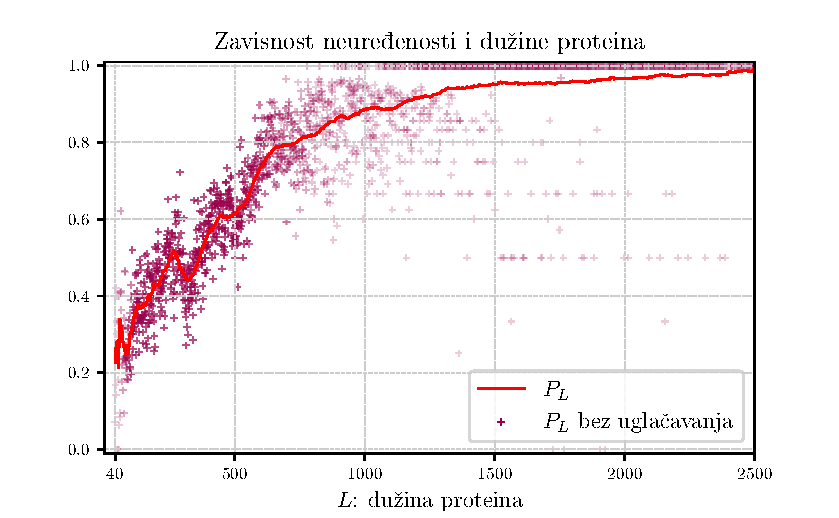
\includegraphics[]{plots/PL_F}
% \decoRule
\caption {
  Zavisnost neuređenosti i dužine CAFA3 proteina minimalne dužine 40 AK
  \footnotesize
  ($P_L$ sa prozorom uprosečavanja podrazumeva $l = 0.1L$, dok
  krstići predstavljaju diskretne vrednosti L za $l = 0$. Transparentnost krstića
  ilustruje brojnost proteina dužine $L$. Ako je krstić transparentan
  znači da sadrži manje od 100 proteina.)
}
\label{fig:PL1}
\end{figure}


Pored gore prikazanog referentnog metoda predložićemo još jedan pristup
procenjivanju veličine $P_L$.
% \keyword{Slučajno generisani} \en{random generated} proteini za procenu $P_L$.
Razmotrićemo dva modela zasnovana na slučajno generisanim proteinima. Prvi,
naivni model \keyword{uniformne verovatnoće} ($P_L uniform$) podrazumeva da se svaka
aminokiselina javlja sa istom verovatnoćom, odnosno $p=1/20$. U statistici je ovaj
model još poznat kao model jednakih verovatnoća \en{equiprobable model, EPM}.
Drugi model koji ćemo zvati \keyword{slučajni ili \textit{random} model}, kraće
RM ($P_L random$)  predstavlja slučajnu promenljivu čija verovatnoća zavisi od učestalosti
aminokiselina iz CAFA3-skupa i prikazana je na Slici \ref{fig:AK_ucestalost}.
% Koristeći ova dva modela za svaki protein generisan je slučajan protein iste
% dužine koji se koristi za procenu $P_L$.
Na osnovu predstavljenih modela definisana su dva nova skupa sekvenci (EPMS i
RMS) iste kardinalnosti kao polazni CAFA3-skup, u kojima su sekvence bile istih
dužina kao u polaznom skupu. U EPMS, sekvence su generisane na osnovu uniformne
raspodele aminokiselina, dok su u RMS sekvence definisane na osnovu učestalosti
aminokiselina iz CAFA3-skupa.


\begin{figure}[th]
\centering
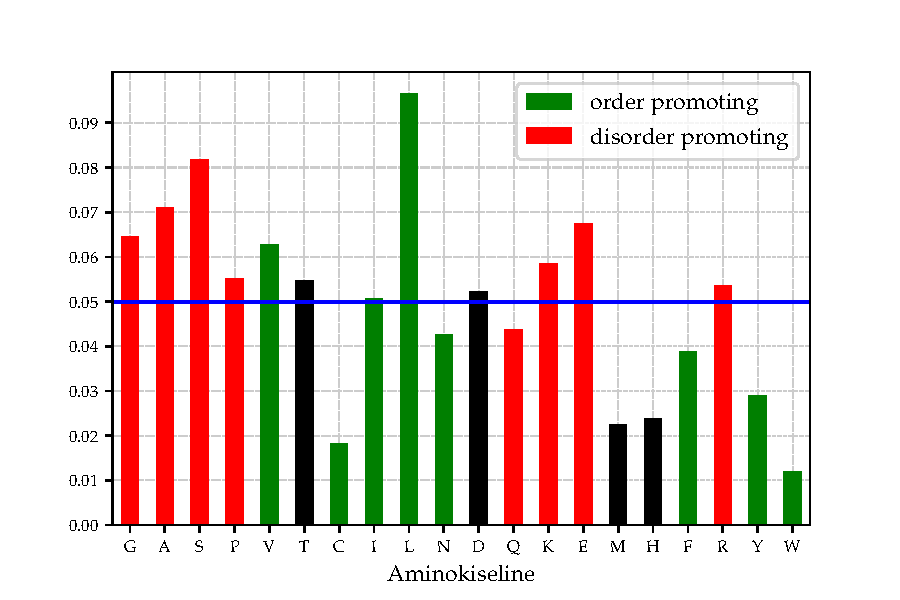
\includegraphics[]{plots/AK_ucestalost}
% \decoRule
\caption{
  Učestalost aminokiselina u CAFA3-podacima
  \\ \footnotesize
  (Učestalost prikazuje slučajni model, dok boja AK obeležava afinitet prema
  uređenosti ili neuređenosti. Aminokiseline su poređane u rastućem poretku
  od najlakše do najteže.) 
}
\label{fig:AK_ucestalost}
\end{figure}

Poređenje predloženih modela sa referentnim $P_L$ prikazano je na Slici
\ref{fig:PL2}. Jasno se vidi da slučajni model predstavlja vizuelno dobru
aproksimaciju dok model uniformne verovatnoće znatno odstupa rastući sporije (naizgled
skoro linearno).
% Kako VSL2b prediktor prepoznaje neuređene regione na osnovu učestalosti
% aminokiselina, ovo ponašanje nije čudno jer je manja verovatnoća pojave
% aminokiselina koje promovišu neuređenost.
Zbog znatnog vizuelnog odstupanja model uniformne verovatnoće nije korišćen u daljoj analizi.


\begin{figure}[th]
\centering
% 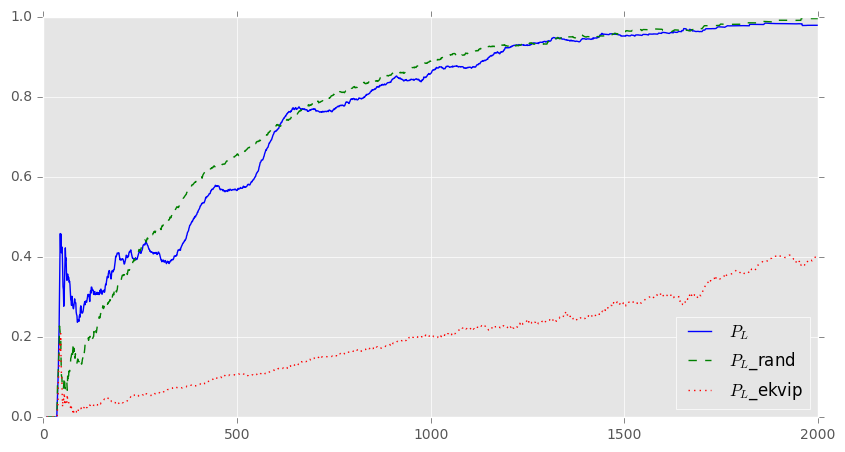
\includegraphics[scale=0.65]{Figures/PL2}
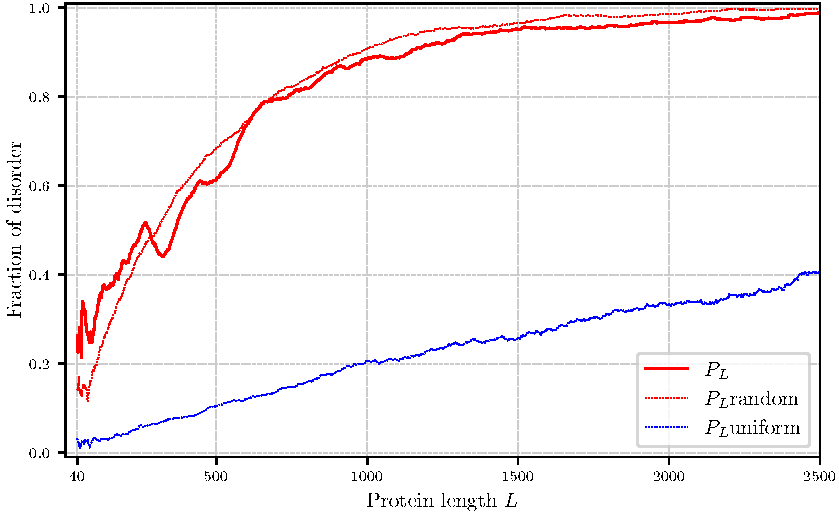
\includegraphics[]{plots/PL_F_cmp}
% \decoRule
\caption{Upoređivanje $P_L$, $P_L random$ i $P_L uniform$ modela nad CAFA3-podacima}
\label{fig:PL2}
\end{figure}


Jedno od objašnjenja zašto je model uniformne verovatnoće naivan i toliko
odstupa od prvobitnog metoda proizilazi iz činjenice da aminokiseline u prirodi
imaju inherentno različitu učestalost. Naime, aminokiseline ne mogu  imati istu
verovatnoću pojavljivanja jer se  broj njihovih kodona razlikuje. Neke
aminokiseline su kodirane sa samo jednim, a druge i sa 6 kodona. Očekivano je
da veći broj kodona povećava učestalost aminokiseline i ta korelacija uz
izuzetke arginina predstavljena je Slikom \ref{fig:aminoacid}
\parencite{AKfrekvencija}.

\begin{figure}[th]
\centering
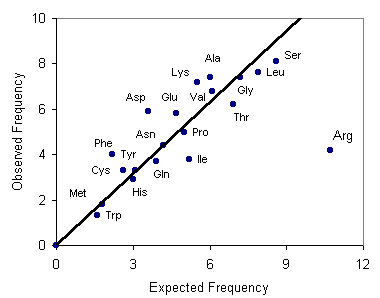
\includegraphics[scale=0.7]{aminoacid}
% \decoRule
\caption{Očekivana i izmerena učestalost aminokiselina kod kičmenjaka (preuzeto sa \cite{AA_freq_link}).  \footnotesize
  Izmerena učestalost dobijena je analizom 53 kompletno sekvencionirana proteina iz kičmenjaka \cite{King1969}.
  Očekivana učestalost kodona izračunata je kao proizvod učestalosti nukleinskih baza koje ga čine.
  Očekivana učestalost aminokiseline je zbir očekivanih učestalosti njenih kodona.
}
\label{fig:aminoacid}
\end{figure}




\clearpage
\label{ocenjivanje}
\subsection{Ocenjivanje zavisnosti funkcije od neuređenosti}

Neka je $S_j$ skup proteina koji imaju pridruženu funkciju $j$. Tada se učestalost
neuređenih proteina u oznaci $F_j$ može izračunati kao:
$$F_j = \dfrac{\sum_{s_i \in S_j} d(s_i)} {|S_j|} $$


\begin{definicija}
  \label{neuredjenost}

  \keyword{Neuređenost} funkcije (GO-termina ili ključne reči) je mera učestalosti
  neuređenih proteina ($F_j$).
\end{definicija}


Nulta hipoteza za $F_j$ je tvrdnja da $F_j$ zavisi samo od dužine sekvence tj. $P_L$. \\
Neka je $X_L$ Bernulijeva slučajna promenljiva oblika $X_L : \begin{pmatrix} 0 & 1\\ P_L & 1-P_L \end{pmatrix}$. \\
Tada nultu hipotezu modeliramo raspodelom $Y_j$, koja za razliku od $F_j$ koristi
slučajnu promenljivu $X_L$ umesto  $d(s_i)$, odnosno:


% Nultu hiptezu koja predviđa da je rezultat $F_j$ posledica samo slučajnosti, to
% jest zavisi samo od $P_L$ opisana je preko slučajne veličine $Y_j$ gde je $X_L$
% Bernulijeva slučajna veličina sa verovatnoćom $P(X_L = 0) = P_L$ odnosno $P(X_L
% = 1) = 1-P_L$

$$ Y_j = \dfrac {\sum_{s_i \in S_j} {X_{|s_j|}}}{|S_j|}$$

Ako $F_j$ izlazi iz intervala poverenja raspodele $Y_j$ onda funkcija $j$
sadrži značajno mnogo predviđenih (ne)uređenih proteina (neuređenost je
statistički značajna).
Preciznije, ako je p-vrednost \en{p-value} manja od 0.05 onda je funkcija $j$
povezana (korelirana) sa neuređenim proteinima, a ako je \textit{p-value} veća
od 0.95 onda je funkcija $j$ povezana (korelirana) sa uređenim proteinima. U
suprotnom, povezanost (koreliranost) funkcije $j$ sa (ne)uređenošću nije
statistički značajna.  

\begin{definicija}
  \label{neuredjena_funkcija}
  Funkcija (GO-termin ili ključna reč) je \keyword{neuređena} ako je povezana
  ($p<0.05$) sa neuređenim proteinima, a uređena ako je povezana ($p>0.95$) sa
  uređenim proteinima.
\end{definicija}

% ----
% U nastavku teksta, pod neuređenošću funkcije, ključne reči ili GO-termina, biće
% podrazumevano da je odgovarajuća p vrednost manja od 0.05. Analogno, pod
% uređenošću funkcije, ključne reči ili GO-termina, biće podrazumevano da je
% odgovarajuća p vrednost veća od 0.95.
% -----
% Kada se kaže da je funkcija, ključna reč ili GO-termin (ne)uređen
% podrazumevaće se da je odgvorajauća p-vrednost manja od $0.05$ ili veća
% od $0.95$.

Zbog matematičkog oblika $X_L$ teško je analitički proceniti $Y_j$ pa se se
pribegava empirijskom računanju p-vrednosti. Empirijska p-vrednost određena je
tako što je za 1000 realizacija $Y_j$ izračunato očekivanje da je realizacija
$Y_j$ veća od $F_j$.
Preciznije, vektor\footnote{zamenili smo skup $S_j$ za vektor $S_j$. Ovo je
implementacioni detalj.} $S_j$ sadrži $k$ proteina $S_j=\{s_1, s_2, ...
,s_{k}\}$.  Protein $s_i$ ima dužinu $L_i$ za koju je izračunata verovatnoća
$P_{L_i}$.  Tada generatorom Bernulijevih slučajnih brojeva, za svaki protein
$p_i$ na osnovu $P_{L_i}$ generišemo realizaciju $X_L$. Rezultat je vektor od
$k$ vrednosti nula ili jedan. Učestalost jedinica u rezultujućem vektoru
predstavlja prvu realizacija $Y_j$.  Postupak se ponavlja 1000 puta i broji
se koliko puta je realizacija $Y_j$ bila veća od $F_j$. Dobijeni zbir deli se
sa 1000 i rezulatat je empirijska p-vrednost.

% \begin{verbatim}
%     p = np.array( [yj>Fj for yj in Yj_1000] ).mean()
% \end{verbatim}

Referentni autori tvrde da se za veće skupove $S_j$, raspodela
$Y_j$ ponaša kao normalna. To znači da se ocena Z-skor može dobiti kao
$Z_j=(F_j-\mu_j)/\delta_j$ gde je $\mu_j$ očekivanje, a $\delta_j$ standardna
devijacija. Onda se Z-skor može koristiti za rangiranje (ne)uređenih funkcija
po statističkoj značajnosti.
\begin{definicija}
  \label{stat_naj}
  \keyword{Statistički najznačajnije} uređene/neuređene funkcije
  (GO-termini ili ključne reči) su one koje imaju najmanji/najviši Z-skor.
\end{definicija}
% Dodatno, p-vrednost može da se aproksimira kao $1/2(1-erf(Z_j/2))$
% \footnote{$erf()$ je gausova funkcija greške,
% $erf(x)=\dfrac{2}{\sqrt{\pi}} \int_{0}^{x}  e^{-t^2} dt$ }
% ako raspodela liči na normalnu. Ovo je nekad korisno jer sa 1000 realizacija
% $Y_j$ nema dovoljnu preciznost za p vrednost manju od $1/1000=0.001$. Međutim u
% ovom radu to nije korišćeno jer su sva sortiranja (kao i u referentnom radu)
% izvršena po Z-skor oceni.


